%From https://egu2018.eu/PICO_how-to_guide_to_PICO.pdf
%Abstracted and templated by Brian Ballsun-Stanton, Macquarie University.
%original template by https://github.com/snowtechblog/pico-latex-presentation by Anselm Köhler

\documentclass[unknownkeysallowed,usepdftitle=false, parskip=full]{beamer}
% unknownkeysallowed is needed for mac and the newer latex version -> is more picky than before...
\usetheme[headheight=1cm,footheight=2cm]{boxes}
%\usetheme{default}


\usepackage{default}
\usepackage{graphicx}
%example pictures created via: http://lorempixel.com/1200/800/cats/Figure2/. Credit to http://lorempixel.com/images.php

%package for media
\usepackage{media9}
\usepackage{epsfig}
\usepackage{siunitx}
\usepackage{color}
\usepackage{ifthen}
%usepackage{ragged2e}

\usepackage[T1]{fontenc}
\usepackage[utf8]{inputenc}
%https://tex.stackexchange.com/a/203804/5483

\usepackage[activate={true,nocompatibility},final,tracking=true,kerning=true,spacing=true,factor=1100,stretch=10,shrink=10]{microtype} % http://www.khirevich.com/latex/microtype/
\microtypecontext{spacing=nonfrench}

\usepackage{lipsum} % for dummy text only
\usepackage[UKenglish]{babel} %https://tex.stackexchange.com/a/27743 
\usepackage[pangram]{blindtext} % https://tex.stackexchange.com/a/48411

%\usepackage{parskip} % from https://tex.stackexchange.com/q/11622
%\setlength{\parskip}{12pt} 

%\setparsizes{\parindent}{12pt}{\parfillskip}

%\usepackage{etoolbox} % as per https://tex.stackexchange.com/a/24331
%\appto\chapterheadendvskip{\vspace{-1\parskip}}
%\setparsizes{\parindent}{50pt plus 20pt minus 30pt}{\parfillskip}

\setbeamertemplate{navigation symbols}{}%remove navigation symbols
\setbeamersize{text margin left=1cm,text margin right=1cm}

% some colors
\definecolor{grau}{gray}{.5}
\definecolor{slfcolor}{rgb}{0,0.6274,0.8353}
\definecolor{wslcolor}{rgb}{0,0.4,0.4}

% setup links
\hypersetup{%
	%linkbordercolor=green,%
	colorlinks=false,%
	pdfborderstyle={/S/U/W 0},%
	%pdfpagemode=FullScreen,%
	pdfstartpage=4%
	}

% setup some fonts
\setbeamerfont{title}{series=\bfseries, size=\small}
\setbeamerfont{author}{size*={5pt}{0pt}}
\setbeamerfont{institute}{size*={3pt}{0pt}}
\setbeamerfont{bodytext}{size=\scriptsize}
	
% Title setup	
\title{Improving the efficiency of textual analysis in R}
\author{Sophie Avard (\texttt{sophie.avard@hdr.mq.edu.au})}
\institute{Macquarie University}
% add title in headbox
\setbeamertemplate{headline}
{\leavevmode
\begin{beamercolorbox}[width=1\paperwidth]{head title}
  % LOGO
  \begin{columns}[t, totalwidth=\textwidth]
  \begin{column}[c]{1.05cm}
     
  \end{column}
  % TITLE
   \begin{column}[c]{10.6cm}
   \centering \usebeamerfont{title} \textcolor{slfcolor}{\inserttitle} \\
   \centering \usebeamerfont{author} \color[rgb]{0,0,0} \insertauthor \\
   \vspace{-0.05cm}
   \centering \usebeamerfont{institute} \insertinstitute
  \end{column}
  % PICTURE
  \begin{column}[c]{1.15cm}
    \hspace{0.005cm}
   
  \end{column}
  \end{columns}
  {\color{slfcolor}\hrule height 1pt\vspace{0.1cm}}
\end{beamercolorbox}%
}

% setup the navigation in footbox
% first set some button colors
\newcommand{\buttonactive}{\setbeamercolor{button}{bg=wslcolor,fg=white}}
\newcommand{\buttonpassive}{\setbeamercolor{button}{bg=slfcolor,fg=black}}
% now set up that the one active one gets the new color.
\newcommand{\secvariable}{nothing}
% therefore we write before each section (well, everything which should be part of the navi bar)
% the variable \secvariable to any name which is in the next function ...
\newcommand{\mysection}[1]{\renewcommand{\secvariable}{#1}
}
% ... compaired to strings in the following navibar definition ...
\newcommand{\tocbuttoncolor}[1]{%
 \ifthenelse{\equal{\secvariable}{#1}}{%
    \buttonactive}{%
    \buttonpassive}
 }
% ... here we start to set up the navibar. each entry is calling first the function \tocbuttoncolor with the argument which should be tested for beeing active. if active, then change color. afterwards the button is draw. so to change that, you need to change the argument in \toc..color, the first in \hyperlink and before each frames definition... A bit messed up, but works...
\newlength{\buttonspacingfootline}
\setlength{\buttonspacingfootline}{-0.2cm}
\setbeamertemplate{footline}
{\leavevmode
\begin{beamercolorbox}[width=1\paperwidth]{head title}
  {\color{slfcolor}\hrule height 1pt}
  \vspace{0.05cm}
  % set up the buttons in an mbox
  \centering \mbox{
    \tocbuttoncolor{abstract}
    \hyperlink{abstract}{\beamerbutton{2 Minute Madness}}
    \tocbuttoncolor{radar}
    \hspace{\buttonspacingfootline}
      \hyperlink{radar}{\beamerbutton{Proof of Concept}}

    \tocbuttoncolor{line}
    \hspace{\buttonspacingfootline}
      \hyperlink{line}{\beamerbutton{Significance}}

    \tocbuttoncolor{slab}
    \hspace{\buttonspacingfootline}
      \hyperlink{slab}{\beamerbutton{Example Code}}
    \tocbuttoncolor{minor}
    \hspace{\buttonspacingfootline}
      \hyperlink{minor}{\beamerbutton{Limitations}}
    \tocbuttoncolor{conclusion}
    \hspace{\buttonspacingfootline}
      \hyperlink{conclusion}{\beamerbutton{Conclusion}}
    % this last one should normaly not be used... it will open the preferences to change the 
    % behaviour of the acrobat reader in fullscreen -> usefull in pico...
    \setbeamercolor{button}{bg=white,fg=black}
    % for presentation
    %\hspace{-0.1cm}\Acrobatmenu{FullScreenPrefs}{\beamerbutton{\#}}
    % for upload
    
     
\Acrobatmenu{FullScreenPrefs}{\vspace{0.3cm}\hspace{0.24cm}\mbox{%
      \includegraphics[height=0.04\textheight,keepaspectratio]{%
	  figure/CreativeCommons_Attribution_License.eps}%
	  }}
   }
    \vspace{0.05cm}
\end{beamercolorbox}%
}


\begin{document}


%%%%%%%%%%%%%%%%%%%%%%%%%%%%%%%%%%%%%%%%%%%%%%%%%%%%%%%%%%%%%%%%%%%%%%%%%%
\mysection{abstract}
%%%%%%%%%%%%%%%%%%%%%%%%%%%%%%%%%%%%%%%%%%%%%%%%%%%%%%%%%%%%%%%%%%%%%%%%%%
\begin{frame}\label{\secvariable}

  \begin{columns}[t]
  %https://tex.stackexchange.com/a/7452/5483
  \begin{column}[c]{0.45\textwidth}
%http://lorempixel.com/1200/800/cats/Figure2/     
%http://lorempixel.com/1200/800/cats/Figure3/

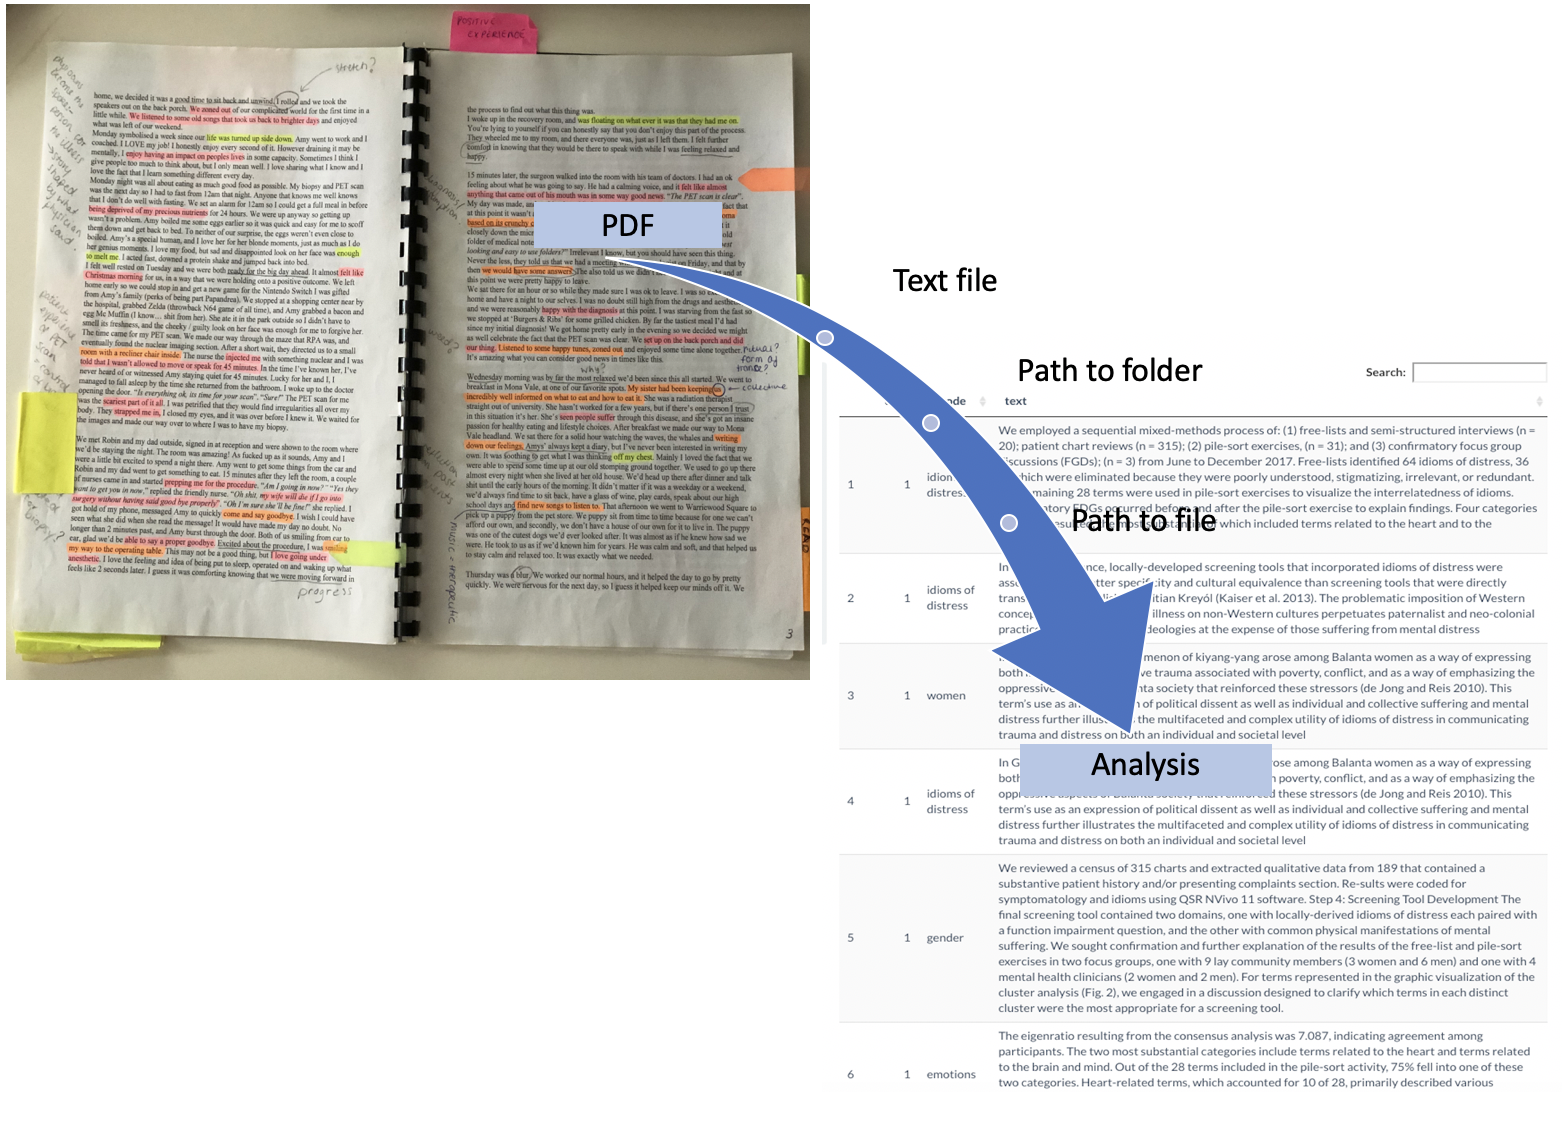
\includegraphics[width=1\textwidth,height=0.5\textheight,keepaspectratio]{poc.png}\\

\textbf{Problem #1:} Unreliable tagging.\\
\textbf{Problem #2:} Documents needed to be in a txt file format.\\
\textbf{Problem #3:} Moving the files into the correct folder was time consuming.\\
    \end{column}
    \begin{column}[c]{0.45\textwidth}
    \parbox{\linewidth}{
    
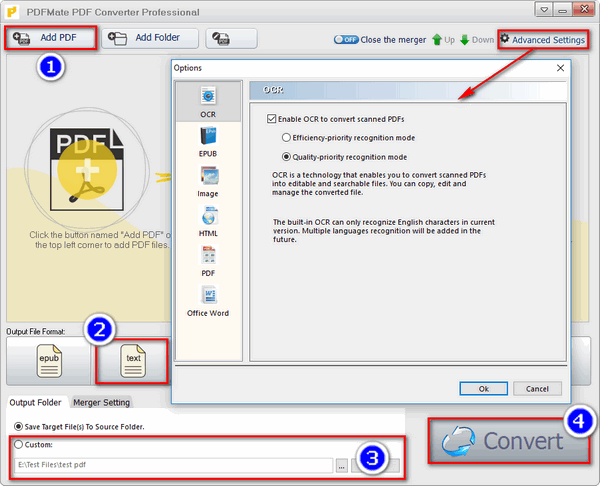
\includegraphics[width=3\textwidth,height=0.5\textheight,keepaspectratio]{pdf-to-txt-steps.png}\\

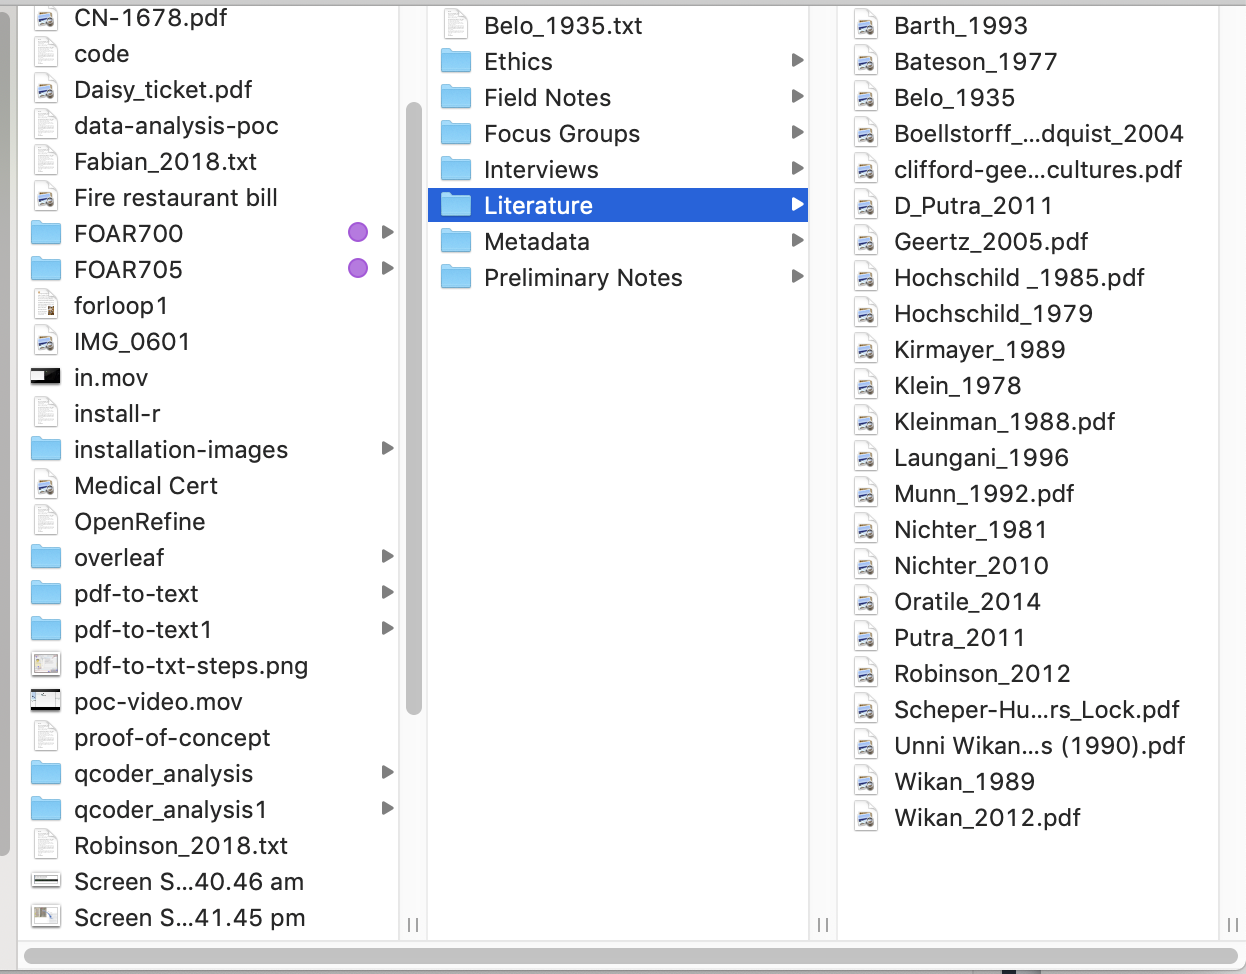
\includegraphics[width=3\textwidth,height=0.5\textheight,keepaspectratio]{literature.png}


      }
    \end{column}
    
  \end{columns}

  
\end{frame}



\begin{frame}\label{\secvariable} %%Eine Folie
\begin{center}
\textbf{Solution}\\
A lightweight and easy-to-use script to make textual analysis in R more efficient. Here's what my solution did!
%http://lorempixel.com/1200/800/cats/Figure5/
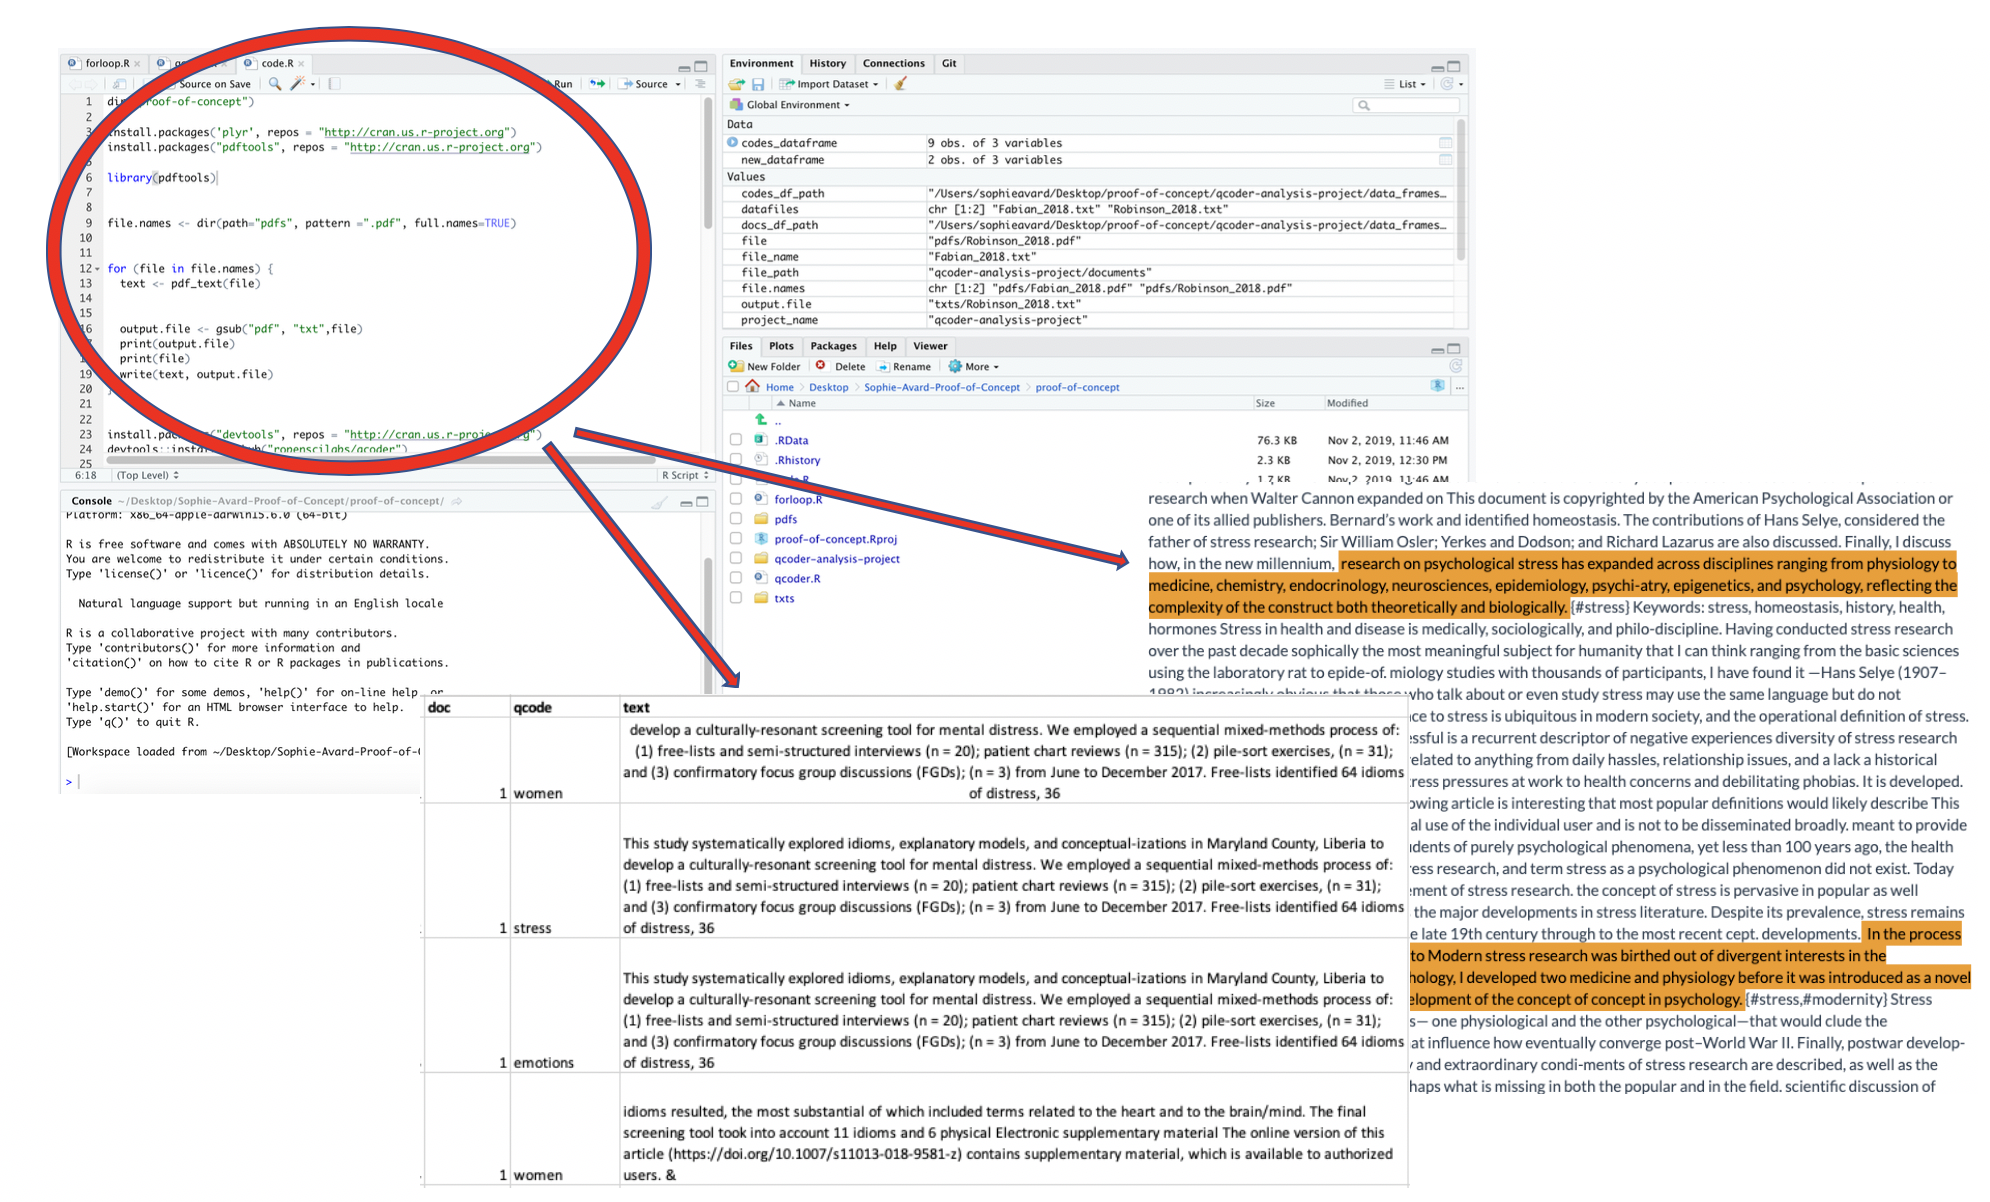
\includegraphics[width=1\textwidth,height=0.8\textheight,keepaspectratio]{figure6.png}
\end{center}

    \parbox{\linewidth}{

}
\end{frame}
%%%%%%%%%%%%%%%%%%%%%%%%%%%%%%%%%%%%%%%%%%%%%%%%%%%%%%%%%%%%%%%%%%%%%%%%%%
\mysection{radar}
%%%%%%%%%%%%%%%%%%%%%%%%%%%%%%%%%%%%%%%%%%%%%%%%%%%%%%%%%%%%%%%%%%%%%%%%%%
\begin{frame}\label{\secvariable}
  \begin{columns}[t]
  %https://tex.stackexchange.com/a/7452/5483
    \begin{column}[c]{0.45\textwidth}
    \parbox{\linewidth}{

      
      
      My proof of concept:
      \begin{enumerate}
          \item converts pdf's to txt files 
          \item Builds a path to the txt files 
          \item Imports the data into qcoder 
          \item Runs qcoder Shiny app for textual analysis
      \end{enumerate}
   
      }
    \end{column}
    \begin{column}[c]{0.45\textwidth}
%http://lorempixel.com/1200/800/cats/Figure2/     
%http://lorempixel.com/1200/800/cats/Figure3/

\includegraphics[width=1\textwidth,height=0.5\textheight,keepaspectratio]{figure7.png}\\
\vspace{12pt}

\includegraphics[width=1\textwidth,height=0.5\textheight,keepaspectratio]{figure8.png}
    \end{column}
  \end{columns}

  
\end{frame}

%%%%%%%%%%%%%%%%%%%%%%%%%%%%%%%%%%%%%%%%%%%%%%%%%%%%%%%%%%%%%%%%%%%%%%%%%%
\mysection{line}
%%%%%%%%%%%%%%%%%%%%%%%%%%%%%%%%%%%%%%%%%%%%%%%%%%%%%%%%%%%%%%%%%%%%%%%%%%
\begin{frame}\label{\secvariable}
\begin{center}
  \vspace{-0.5cm}
  %http://lorempixel.com/1200/800/cats/Figure4/
 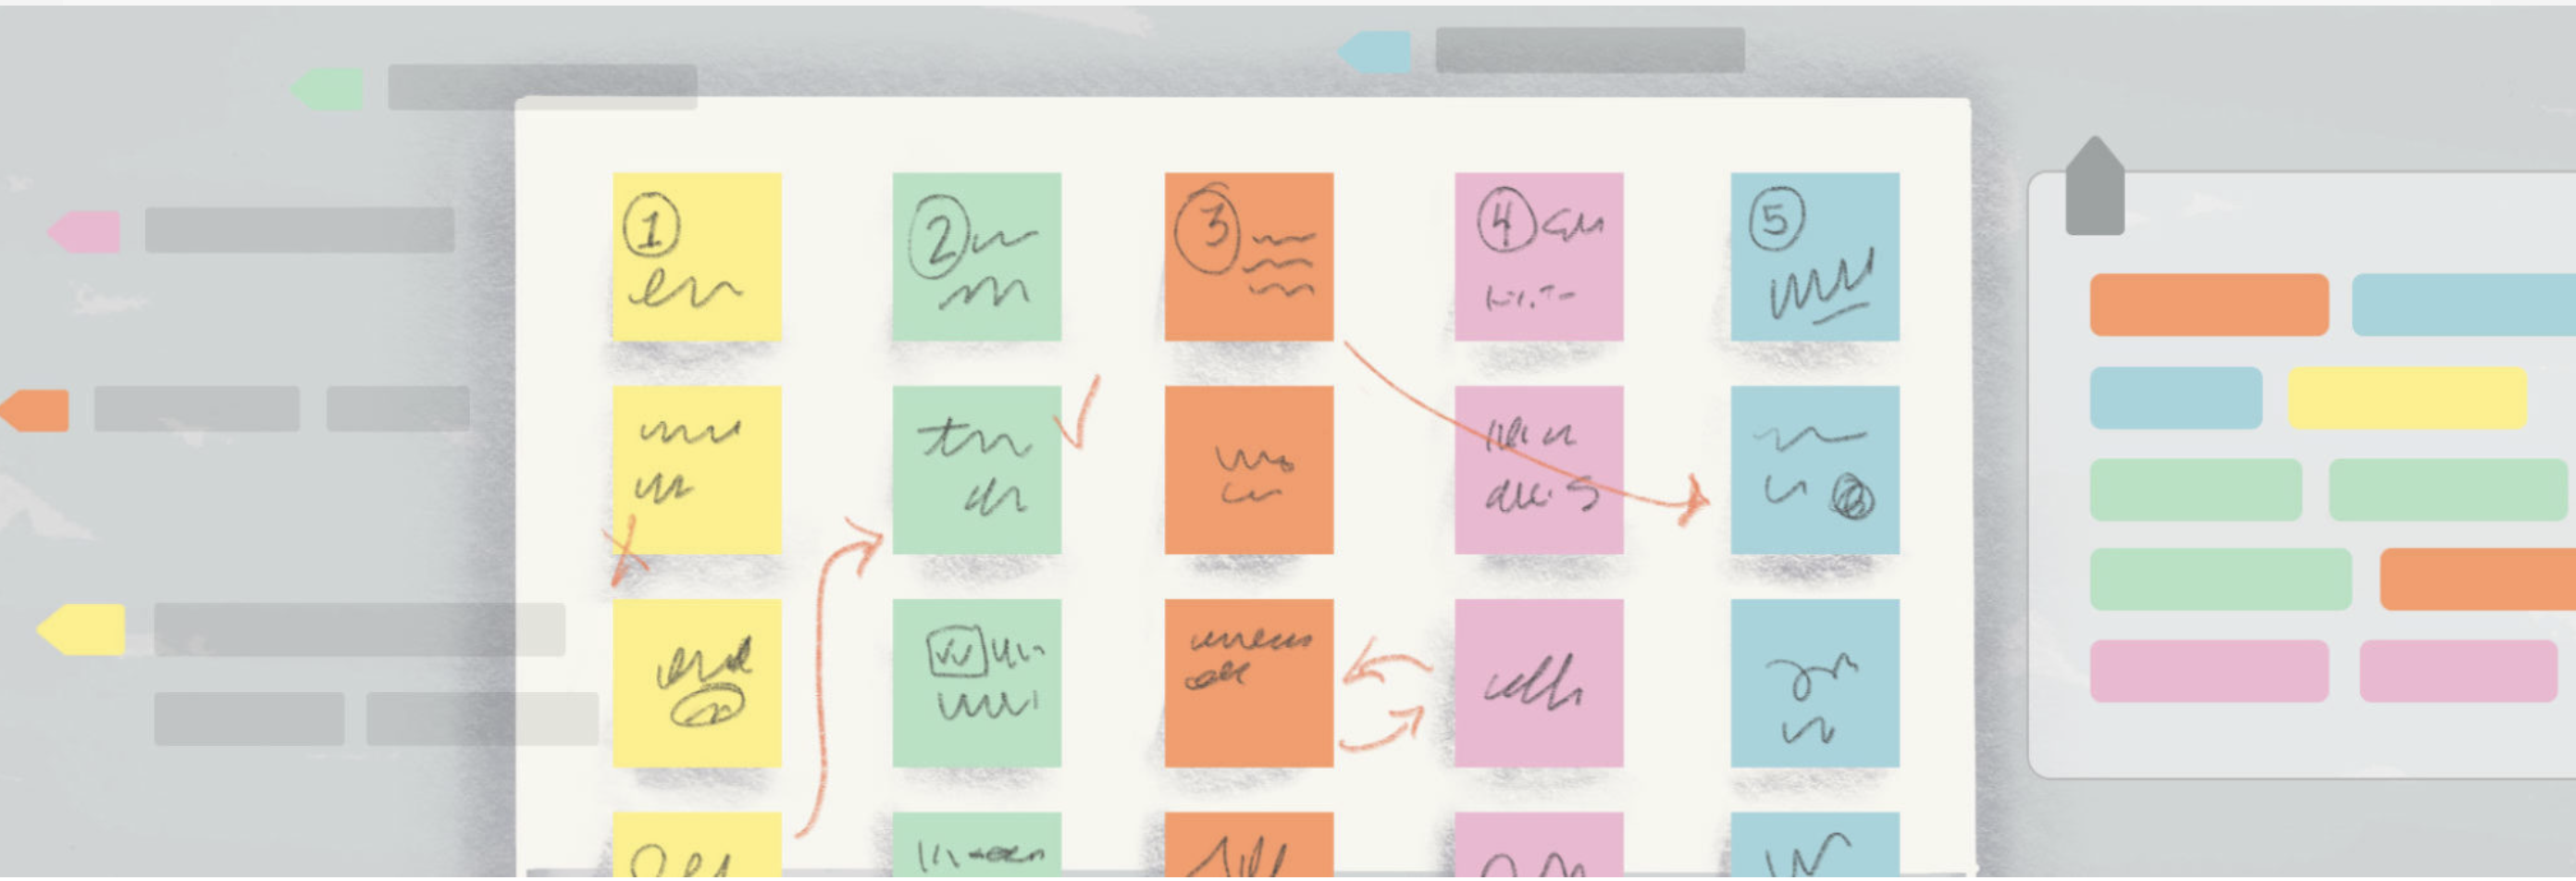
\includegraphics[width=1\textwidth,height=0.75\textheight,keepaspectratio]{figure10.png}
\end{center}
  \vspace{-0.5cm}
  
  \textbf{Significance}
  \begin{enumerate}[(a)]
  \item Able to manage large amounts of data 
  \item Greater flexibility and thoroughness - add codes, define codes, search data. 
  \item Reduces the time spent converting and moving files 
  \item Supports other data analysis packages in R
  \end{enumerate}

  %$\quad \Rightarrow$ Aliquam et turpis eget lacus finibus congue.
  
\end{frame}

%%%%%%%%%%%%%%%%%%%%%%%%%%%%%%%%%%%%%%%%%%%%%%%%%%%%%%%%%%%%%%%%%%%%%%%%%%

\mysection{slab}
%%%%%%%%%%%%%%%%%%%%%%%%%%%%%%%%%%%%%%%%%%%%%%%%%%%%%%%%%%%%%%%%%%%%%%%%%%
\begin{frame}\label{\secvariable}
%http://lorempixel.com/1200/800/cats/Figure6/
\begin{center}
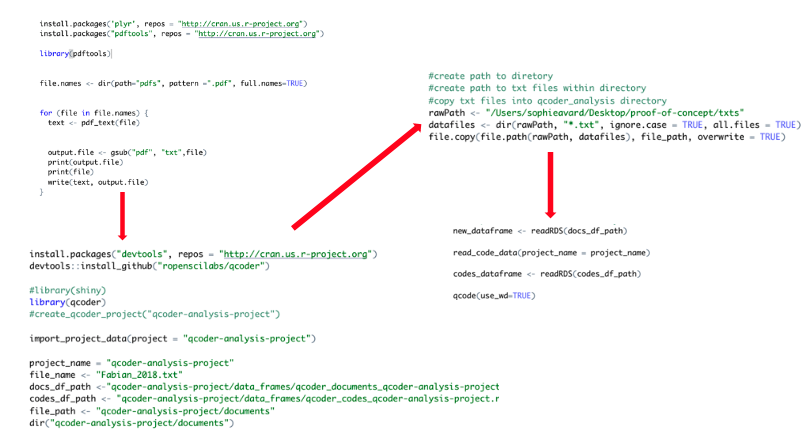
\includegraphics[width=1\textwidth,height=0.75\textheight,keepaspectratio]{figure5.png}
\end{center}
    \parbox{\linewidth}{
 \hyperlink{slabtable}{\beamerbutton{more \dots}}
}

\end{frame}



\begin{frame}\label{slabtable}
\begin{columns}
\begin{column}[t]{1.1\textwidth}
\hyperlink{slab}{\beamerbutton{\dots back to figure}}\\

If the script is successful, the qcoder app should automatically open on the users computer. The user then should be able to open their project directory and begin tagging their data. 

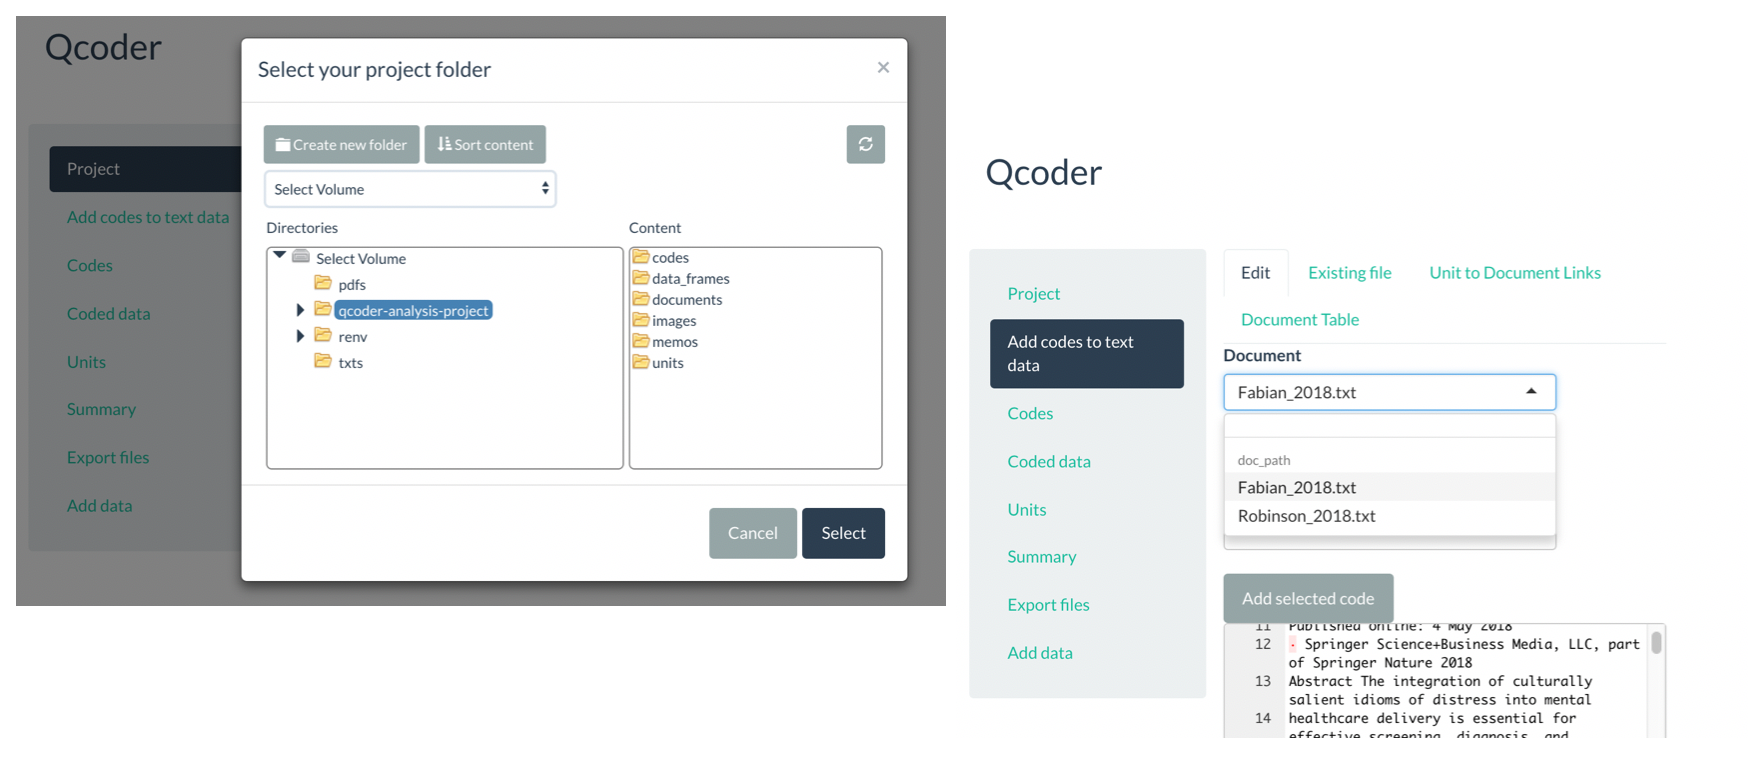
\includegraphics[width=1\textwidth,height=0.7\textheight,keepaspectratio]{qcoder.png}


%Table from original template.

\vspace{0.3cm}
\end{column}
\end{columns}
\usebeamerfont{bodytext}



\end{frame}




%%%%%%%%%%%%%%%%%%%%%%%%%%%%%%%%%%%%%%%%%%%%%%%%%%%%%%%%%%%%%%%%%%%%%%%%%%
\mysection{minor}
%%%%%%%%%%%%%%%%%%%%%%%%%%%%%%%%%%%%%%%%%%%%%%%%%%%%%%%%%%%%%%%%%%%%%%%%%%

\begin{frame}\label{\secvariable}

%

\includegraphics[width=0.45\textwidth,height=1\textheight,keepaspectratio]{figure4.png}\hspace{.05\textwidth}
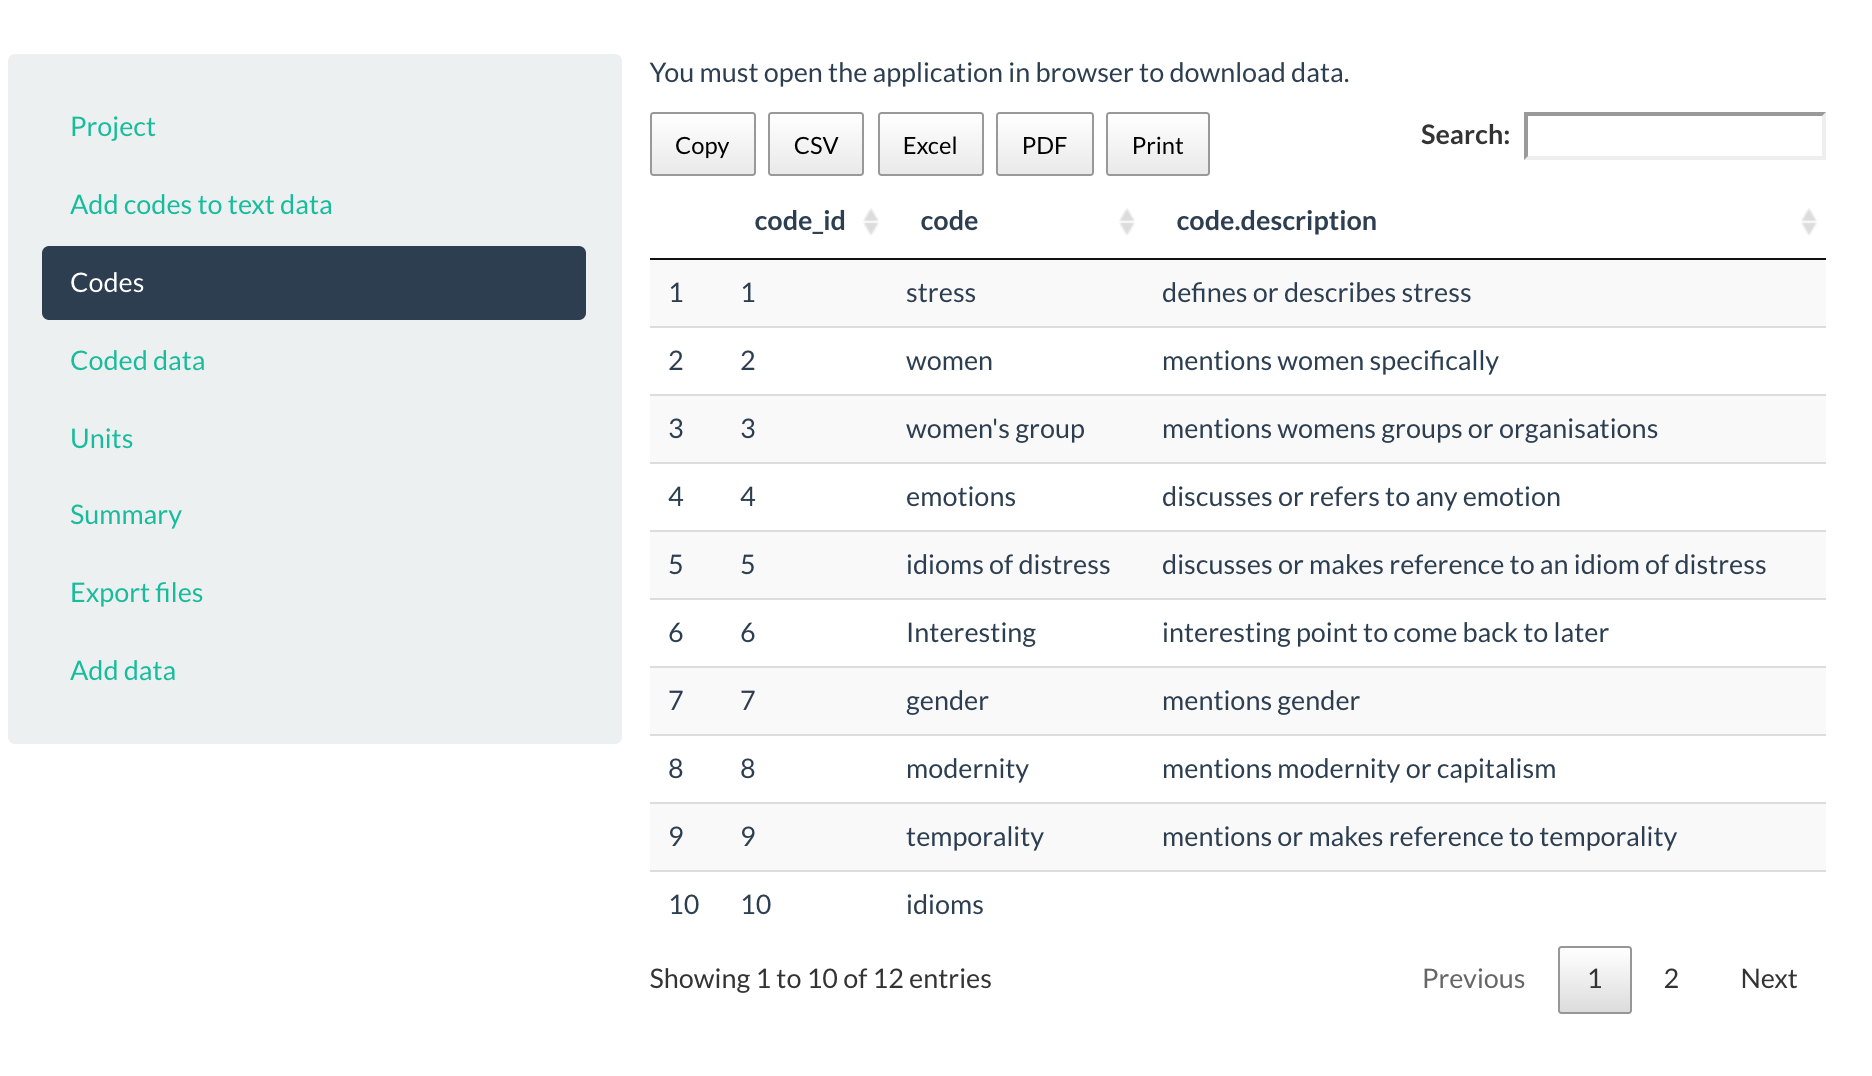
\includegraphics[width=0.45\textwidth,height=1\textheight,keepaspectratio]{figure11.png}

Limitations
\begin{itemize}
    \item Cannot add notes or memos to the data during analysis
    \item Due to a bug in the qcoder package, data must be coded and downloaded in one session
    \item Cannot export the highlights from qcoder
\end{itemize}

\end{frame}
%%%%%%%%%%%%%%%%%%%%%%%%%%%%%%%%%%%%%%%%%%%%%%%%%%%%%%%%%%%%%%%%%%%%%%%%%%
\begin{frame}

Proof of concept repository: \href{https://github.com/MQ-FOAR705/Sophie-Avard-Proof-of-Concept}{https://github.com/MQ-FOAR705/Sophie-Avard-Proof-of-Concept}

    
\end{frame}

\end{document}
